\section{Appendix}

\begin{frame}
    \begin{center}
        \LARGE Appendix
    \end{center}
\end{frame}

\subsection{その他の主な結果}


\begin{frame}{位相シフトのない周期外力を持つ Rössler モデル}  
    \begin{minipage}{0.59\textwidth}
        \vspace{0.5em}
        \begin{figure}
                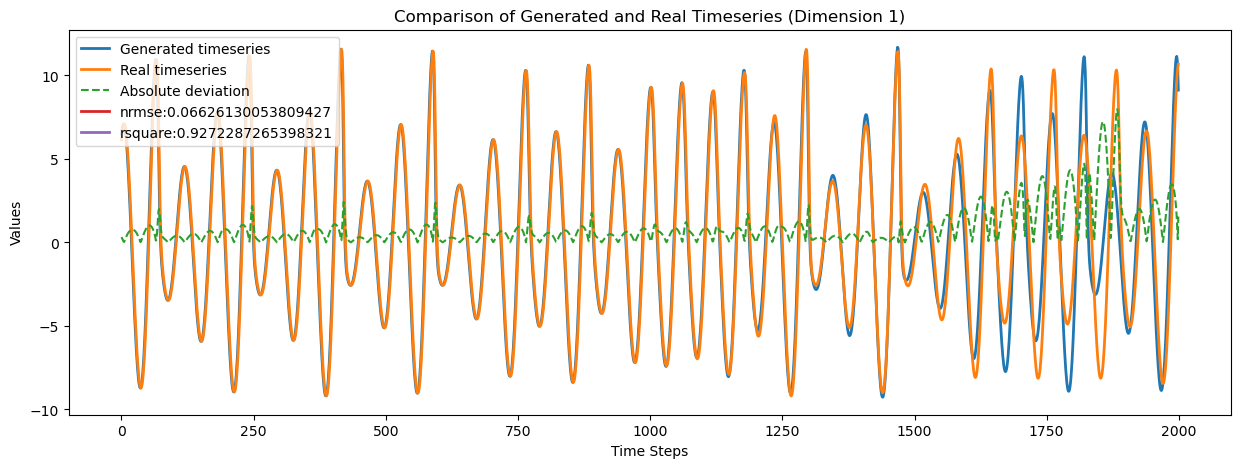
\includegraphics[width=0.7\textwidth]{Fig/rossler_+sin_1.png}
                \label{rossler_+sin_1.png} % ラベルを付ける(参照する場合に使用)
            \end{figure}
            \vspace{-1.0cm}
            \begin{figure}
                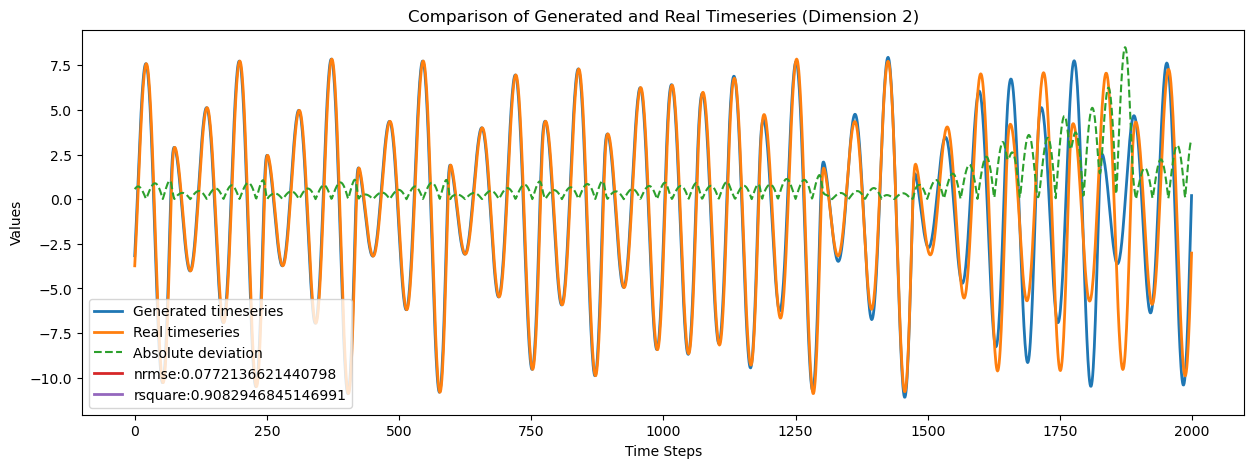
\includegraphics[width=0.7\textwidth]{Fig/rossler_+sin_2.png}
                \label{rossler_+sin_2.png} % ラベルを付ける(参照する場合に使用)
            \end{figure}
            \vspace{-1.0cm}
            \begin{figure}
                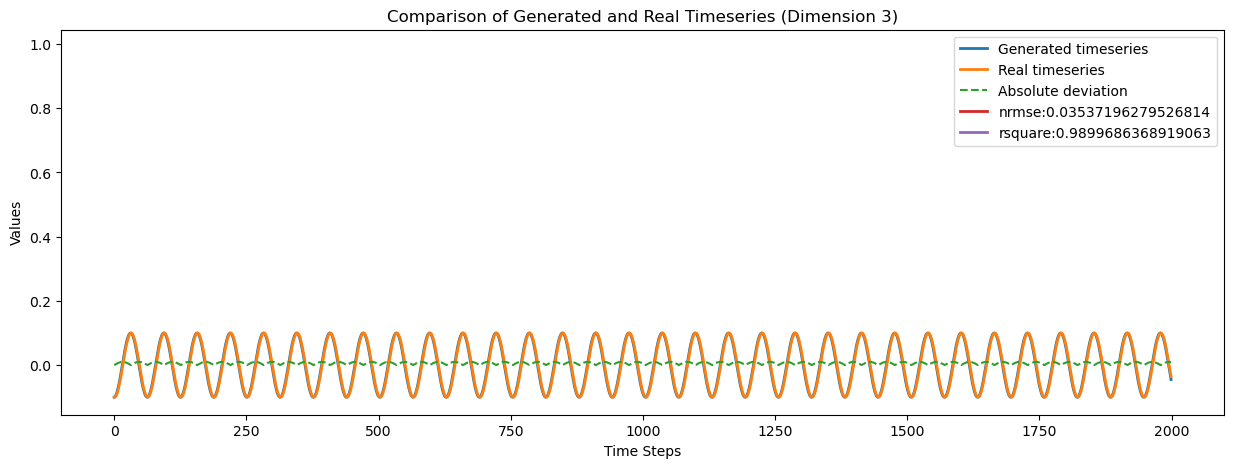
\includegraphics[width=0.7\textwidth]{Fig/rossler_+sin_3.png}
                \vspace{-.3em}
                \caption{位相シフトのない周期外力を持つ Rössler モデル}
                \label{rossler_+sin_3.png} % ラベルを付ける(参照する場合に使用)
            \end{figure}
        \end{minipage}
        \begin{minipage}{0.4\textwidth}
            連立微分方程式:
            \begin{align}
                \frac{dx}{dt} &= -y - z + A \sin(t)\\
                \frac{dy}{dt} &= x + ay \\
                \frac{dz}{dt} &= b + z(x - c)
            \end{align}
            \vspace{-.5cm}
            \begin{itemize}
                \item 外力の振幅$A = 0.1$,変数$a = 0.2,\ b = 0.2,\ c = 5.7$,初期条件$ \left[ x, y, z \right] = [1.0, 1.0, 1.0]$.時間範囲:$[0, 2510]$, 系の周期は $2\pi$ .
            \end{itemize}
        \end{minipage}
\end{frame}

\begin{frame}{確定的な位相シフトの周期外力を持つVan Der Pol モデル}    
    \begin{minipage}{0.49\textwidth}
        
        \vspace{0.5em}
            \begin{figure}
                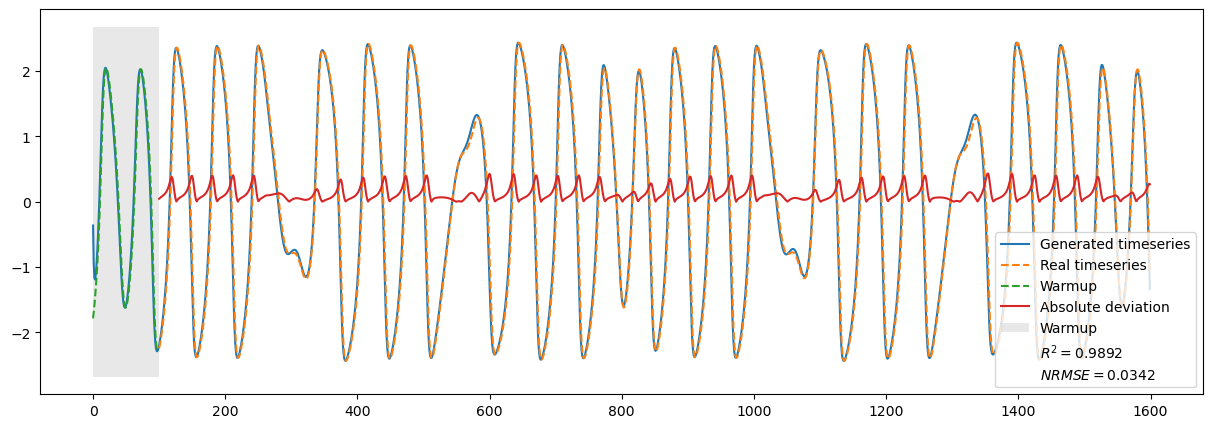
\includegraphics[width=0.8\textwidth]{Fig/output1.png}
                \label{rossler_+sin_alt_dshift_1.png} % ラベルを付ける(参照する場合に使用)
            \end{figure}
            \vspace{-1.0cm}
            \begin{figure}
                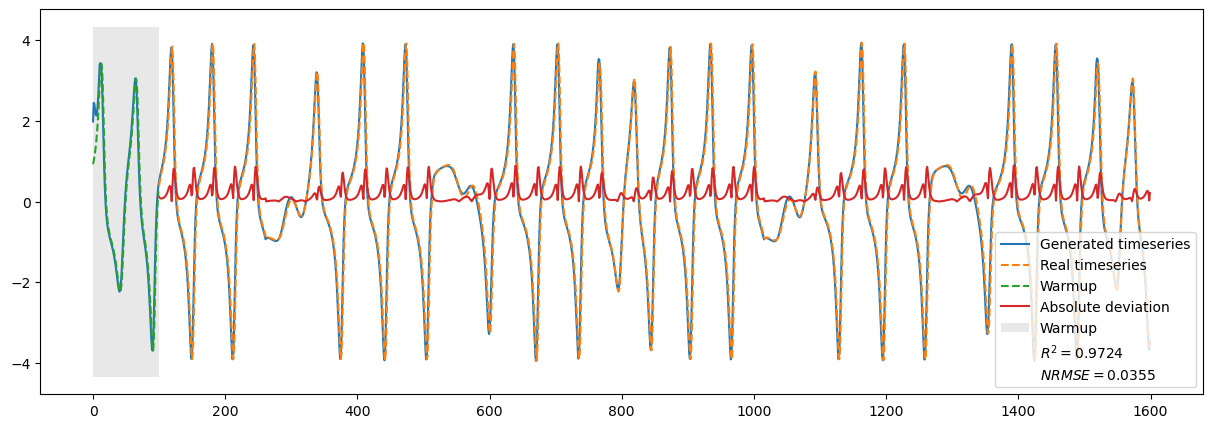
\includegraphics[width=0.8\textwidth]{Fig/output2.png}
                \label{rossler_+sin_alt_dshift_2.png} % ラベルを付ける(参照する場合に使用)
            \end{figure}
            \vspace{-1.0cm}
            \begin{figure}
                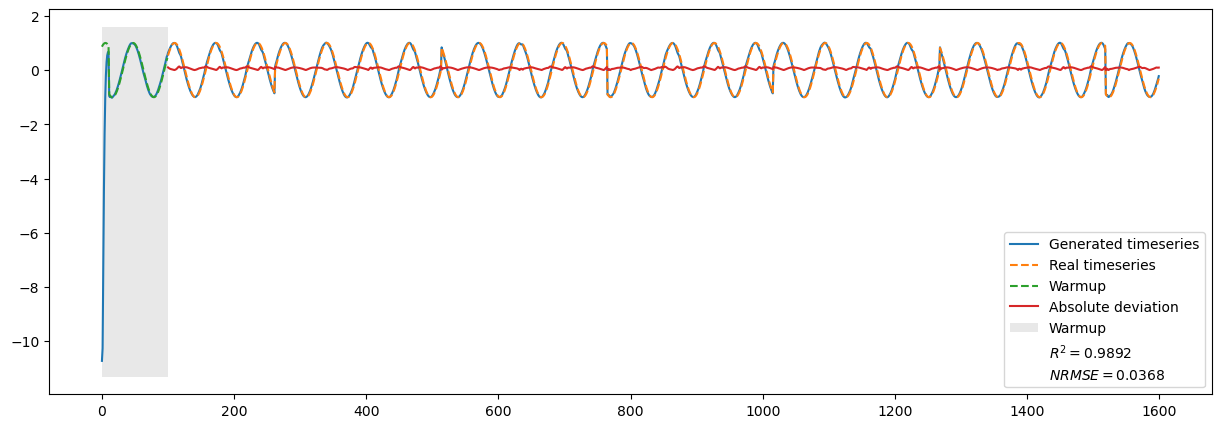
\includegraphics[width=0.8\textwidth]{Fig/output3.png}
                \label{rossler_+sin_alt_dshift_3.png} % ラベルを付ける(参照する場合に使用)
            \end{figure}
            \vspace{-1.0cm}

        \end{minipage}
    \begin{minipage}{0.5\textwidth}
    \end{minipage}
\end{frame}


\subsection{ReservoirPy (v0.3.10)}
\begin{frame}{ReservoirPy (v0.3.10)}

\end{frame}


\subsection{Hyperparameters の最適化}

\begin{frame}{Hyperparameters の最適化 (1/2)}
    アルゴリズムの話.
\end{frame}

\begin{frame}{Hyperparameters の最適化 (2/2)}
    Hyperopt と Optuna の話.
\end{frame}

\subsection{先行研究}  



\begin{frame}{Y. C. Lai et al. (2022) の結果 (1/2)}
    Reservior Computer は Input, Hidden, Output の三つの層から構成される.
    \begin{block}{Reservior Computer の構成:Y. C. Lai et al. (2022)}
    \vspace{0.1cm}
        \begin{minipage}{0.4\textwidth}
            \begin{figure}
                %\centering % 画像を中央揃えにする(オプション)
                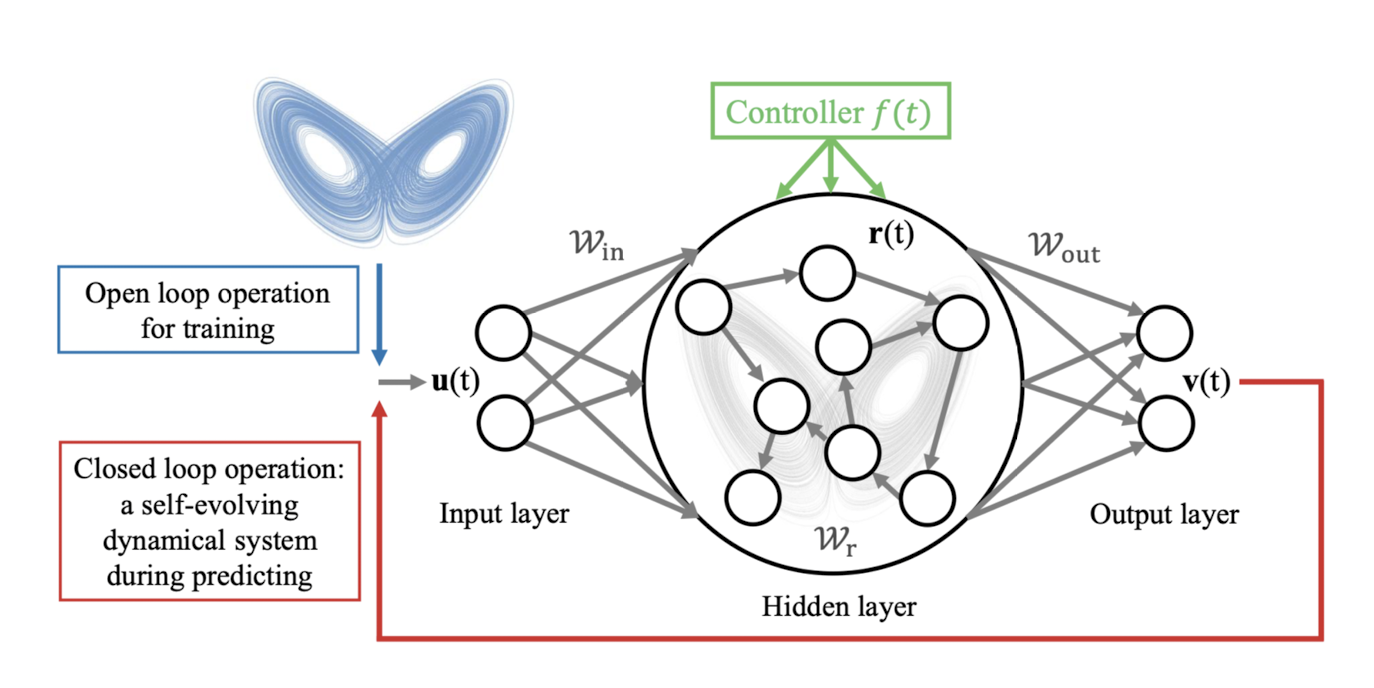
\includegraphics[width=\textwidth]{Fig/Fig.1_Lai.png}
                \caption*{Fig.1 from Y. C. Lai et al. (2022)}
                \label{Fig.1_Lai.png} % ラベルを付ける(参照する場合に使用)
            \end{figure}
        \end{minipage}%
        \begin{minipage}{0.6\textwidth}
            \begin{itemize}
                \item $\mathbf{u}(t) \in \R^{D_{\text{in}}}$: input signal. 
                \item $\mathbf{r}(t) \in \R^{D_r} $: hidden layer state vector.
                \item $f(t)$: (control) external driving signal.  
                \item $\mathcal{W}_{\text{in}} \in D_r \times D_{\text{in}}$: Weighted input matrix.  
                \item $\mathcal{W}_c$: Controller matrix.
                \item $ \mathcal{W}_r \in D_r \times D_{r}$: Weighted network matrix inside.
                \item $\mathcal{W}_{\text{out}}: D_{\text{out}} \times D_{r}$: Output weighted matrix.
            \end{itemize}
    \end{minipage}
    \end{block}
    $\mathbf{u}(t)$ に時系列モデル(low/high-dimensional Lorenz-96 climate network, driven chaotic laser systemなど),$f(t)$にはsinusoidal関数などを使用する(e.g. $f(t) = A \sin (\Omega t) + F$).
\end{frame}

\begin{frame}{Y. C. Lai et al. (2022) の結果 (2/2)}
    学習期間全体の $\mathbf{u}(t)$,全期間の $\mathbf{v}(t)$ を記録する行列をそれぞれ $\mathcal{R'}, \mathcal{V}$ とする.
    \begin{itemize}
        \item $\mathcal{W}_{\text {in }}, \mathcal{W}_c, \mathcal{W}_r$ は Reservior の学習に前もってランダムに定められる.
        \item 学習期間において,$\mathbf{u(t)}$ と $f(t)$ の実データが入力される.
        学習期間の後のself-evolving 期間では,Reservior による出力 $\mathbf{v}(t)$ と $f(t)$ の実データが予測の入力に用いられる.
        \begin{itemize}
            \item $\mathbf{r}(t)$ は 学習期間,self-evolving 期間においてそれぞれ次の式で決定される.
            \vspace{-.2cm}
            \begin{align}
                \mathbf{r}(t+\Delta t) & =(1-\alpha) \mathbf{r}(t) + \alpha \tanh \left[\mathcal{W}_r \mathbf{r}(t)+\mathcal{W}_{\text {in }} \mathbf{u}(t)+\mathcal{W}_c f(t)\right] \label{Lai_r1}\\
                \mathbf{r}(t+\Delta t) & =(1-\alpha) \mathbf{r}(t) + \alpha \tanh \left[\mathcal{W}_r \mathbf{r}(t)+\mathcal{W}_{\text {in }} \mathcal{W}_{\text {out }} \mathbf{r}^{\prime}(t)+\mathcal{W}_c f(t)\right]\label{Lai_r2}
            \end{align}
        \end{itemize}
        \item 複数の $f(t)$ に対して Reservior を sequential に学習させることで,未知の外力がある場合でも予測できるようにする.また,Hyperparameter に関する最適化を行う(後述).
        \item Reservoir に次式における$\mathcal{V}, \mathcal{R'}$ 間のLinear Regressionを通じて$\mathcal{W}_{\text {out }}$ を学習させる.
        \vspace{-.2cm}
        \begin{align}
            \mathcal{W}_{\text {out }}=\mathcal{V} \cdot \mathcal{R}^{\prime T}\left(\mathcal{R}^{\prime} \cdot \mathcal{R}^{\prime T}+\beta \mathcal{I}\right)^{-1}
        \end{align}
    \end{itemize}

\end{frame}

\begin{frame}{理論的な展開}
    Resrvoir Computerの理論的な研究としては Bollt (2021) の研究などが挙げられる.
    \begin{block}{Bollt (2021)}
        Reservoir Computer の activation function (式 \eqref{Lai_r1}, \eqref{Lai_r2} における $\tanh$ 関数)を局所的に線型 activation function $q:\R \ni s \mapsto s \in \R$ とみなすことで,Reservoir 内のダイナミクスに関して次のを得る. \vspace{-.5cm}
        \begin{align}
            \mathbf{v}_{l+1} = \mathbf{W}^{\text {out }} \sum_{j=1}^{\ell} \mathbf{A}^{j-1} \mathbf{W}^{\text {in }} \mathbf{u}_{\ell-j+1} \label{Bollt_eq}
        \end{align}
        式\eqref{Bollt_eq} が VAR(NVAR) の係数行列を表すものだとみなせる.
    \end{block}

\end{frame}


\section{参考資料}
\begin{frame}{参考資料}
    \begin{minipage}{0.49\textwidth}
        \begin{itemize}
            \item Bollt, E. On explaining the surprising success of reservoir computing forecaster of chaos? The universal machine learning dynamical system with contrast to VAR and DMD. \textit{Chaos}, 31(1), 013108 (2021). 
        \end{itemize}    
    \end{minipage}
    \begin{minipage}{0.5\textwidth}
        \begin{itemize}
            \item Kong, L.-W., Weng, Y., Glaz, B., Haile, M., and Lai, Y.-C. Digital twins of nonlinear dynamical systems. arXiv:2210.06144 (2022).
        \end{itemize}
    \end{minipage}
\end{frame}

